\section{Dataset Analysis}
The first step was performing an analysis of the data to understand which patterns could leverage our learning methods. Plotting graphs of the traffic from a few pages we observesd that different pages show remarkably different trends in traffic. This suggests that a good model needs to explicitly distinguish pages.
For specific pages we note a strong year-to-year autocorrelation. We also observed weaker week-to-week and month-to-month trends. One clear example of this case was the Thanksgiving holiday page that showed an yearly spike around a Wednesday on late November, around the date of the holiday.

\begin{figure}[h!]
  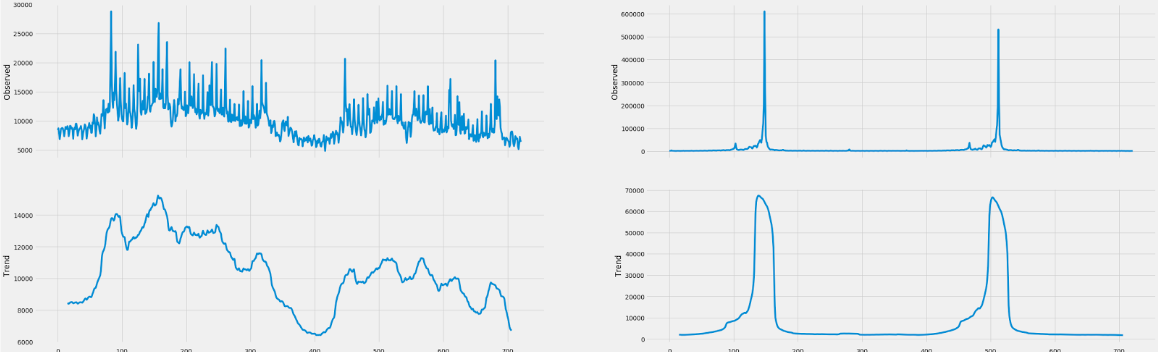
\includegraphics[width=\linewidth]{analysis1.png}
  \caption{Observed Traffic and Traffic Trend from two different pages}
  \label{fig:analysis1}
\end{figure}

Additionally, we have to deal with spikes intraffic not following a regular pattern. We note a short-term dependency following those spikes, which means the days immediately before the prediction are important to consider.


